\chapter{Recursive Jigsaw Reconstruction}
\label{chap:jigsaw}

%\section{Introduction to Recursive Jigsaw Algorithm on Events with $\MET$}
%\label{Jigsaw:Intro}

%\indent Every search involving missing energy has to contend with the fact that information about the invisible system is lost.  The question of how to best fill the missing degree of freedom is a problem ubiquitous to all analysis that have $\MET$ especially when there exists multiple invisible particles in the event. The recursive jigsaw method aims to compartmentalize the lost information and gain the most from what information that is available.\\

%\indent Traditional edge variables such as $M_{T2}$, shown in equation \ref{eqnMT2}, extremize over all possible kinematic configurations of the two invisible particles ${\bf p}_1$ and ${\bf p}_2$.  These variables can form an edge corresponding to some kinematic limit. $M_{T2}$ effectively extremizes over all possible configurations allowed by the missing degrees of freedom.  However, optimizing over too large a phase space can unintentionally destroy useful information.  \\

%\begin{equation}
%\label{eqnMT2}
%M^{2}_{T2} \equiv \mymin[\slashed{\bf p}_{1}+\slashed{\bf p}_{2}=\slashed{\bf E}_{T}^{miss}]  \Big[ \mymax[] \{ m_{T}^{2}({\bf p}_{Tl-},\slashed{\bf p}_{1}), m_{T}^{2}({\bf p}_{Tl+},\slashed{\bf p}_{2})\} \Big]
%\end{equation}

%\indent The recursive jigsaw reconstruction (RJR) method also uses maximizations and minimizations to pin down the missing degrees of freedom.\cite{JigsawCompressed,JigsawContraBoost}  However, these extremizations are restricted to be in a specific location of the decay tree.  \\

%\indent For example, consider a simple particle decay chain where $a \rightarrow b~c$ and then $c \rightarrow 1~2$.  Recursive jigsaw would treat the situation differently if particle $1$ was invisible compared to if particle $b$ was invisible.  To zeroth order, losing information about particle $1$ affects only half the information on particle $c$ which contains only half the information of particle $a$, but losing information on particle $b$ directly affects half the information on particle $a$.   Unlike traditional methods which extremizes over all possible configurations of the invisible particle. RJR compartmentalizes the lost information and extracts the maximum amount of information from events with missing energy.  \\

%\indent RJR separates the event according to a predefined "decay tree."  The decay tree can be as detailed as needed be, either attempting to resolve every branch in the decay tree down to the level of the final state objects or forming aggregate states that have useful kinematics.   Each node in the decay tree represents a particular intermediate state or final state.  RJR will classify all accepted objects into the different nodes by extremizing certain metrics such as the state's mass and the state's energy.  Specifics on the metrics used for each node are detailed in section \ref{Jigsaw:ISR}.  The extremizations set the unknown degree of freedoms in their respective center of mass frames.  The result is then propagated back up the tree to the lab frame, creating a complete picture of the event with all ambiguities resolved.\\

%\indent For the compressed region, the most basic tree involves separating the event into sparticle and ISR systems and then further separating the sparticle system into visible and invisible parts. The decay tree is represented in Figure.~\ref{fig:DecayTree}.  Further detail can be added to the sparticle system such as resolving the stop decays.  For this analysis, we found that attempting to reconstruct individual tops did not result in higher analysis sensitivity.   The high multiplicity of hadronic jets makes reconstructing low pt tops very difficult in signal and gives little separation power because the dominant background is SM $\ttbar$ which also has real tops.  Therefore, we avoid further resolving the sparticle node to the level of individual tops. \\

%\begin{figure}[h]
%\centering
%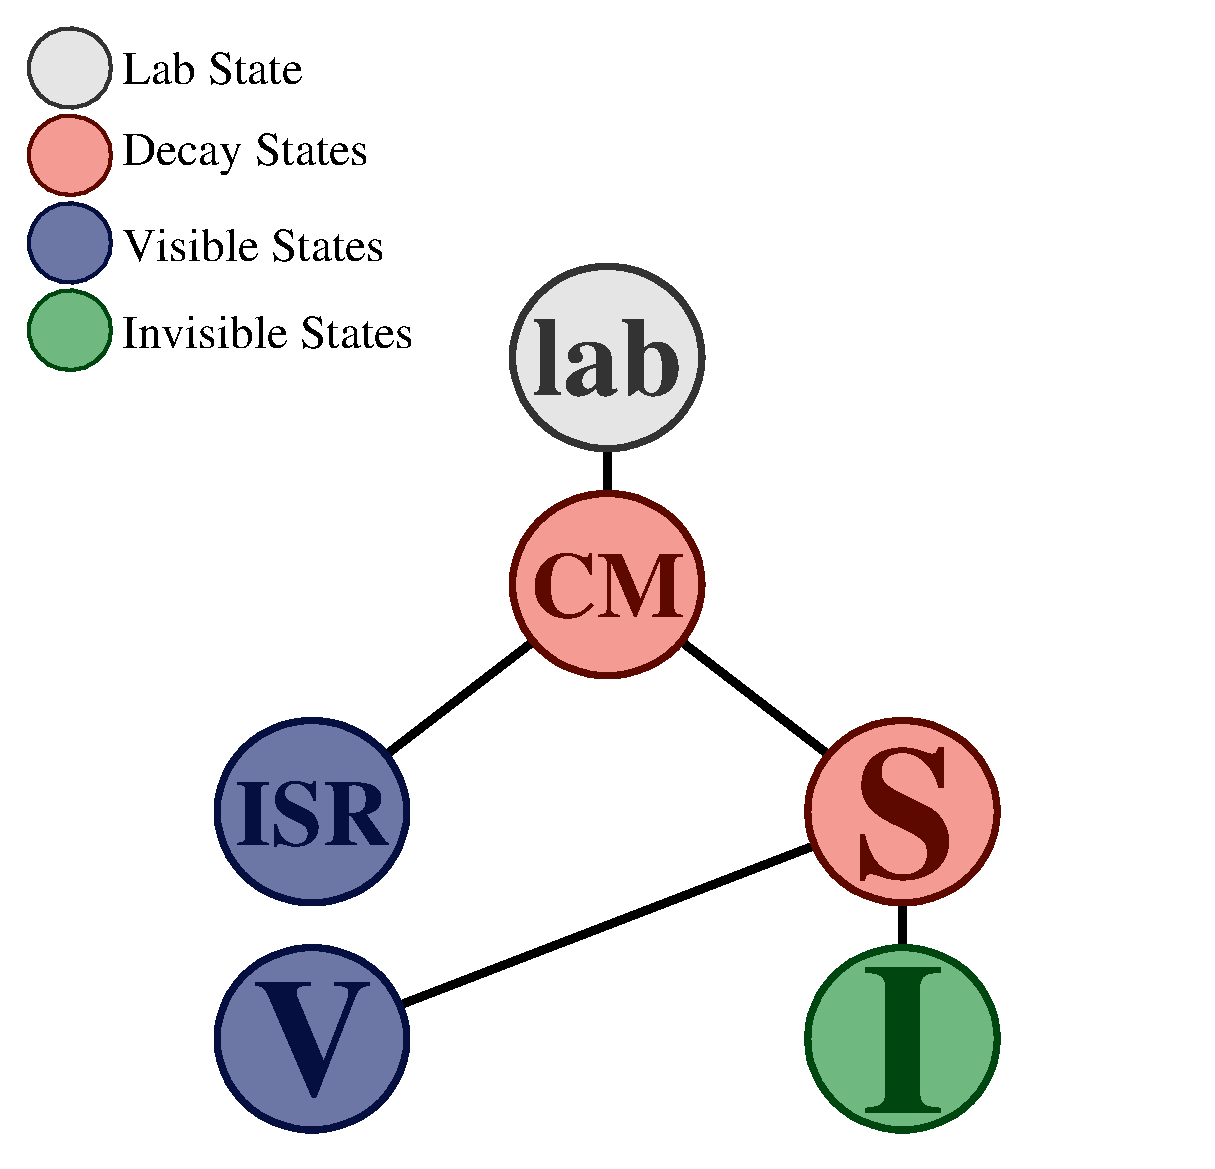
\includegraphics[width=0.6\textwidth]{./figures/strategy/DecayTree.eps}
%\caption{Decay Tree corresponding to ISR-assisted $\MET$ signal analysis strategy. \label{fig:DecayTree}}
%\end{figure}

\indent Every search involving $\met$ has to contend with the fact that information about the invisible system is lost.  The $\met$ reconstruction doesn't capture information on the invisible system's mass or the z component of the momentum.  If multiple energetic weakly interacting particles exist in the event, we cannot directly determine how many energetic weakly interacting particles there are or how the $\met$ should be split among them.  In summary, the question of how best to constrain these missing degrees of freedom is a problem ubiquitous to all analyses that use $\MET$. \\

\indent  For the purpose of this analysis, we aim to separate the event into a sparticle system and an ISR system.  The sparticle system contains objects that originate from stop decays and the ISR system contains ISR jets. \\

\indent We cannot reconstruct the stops directly because we don't have the full four momenta of the two neutralinos.  Therefore, features such as the stop mass peak are of limited use for determining if a jet originated from a stop decay. The high jet multiplicity also makes reconstructing tops very difficult.  Furthermore, top reconstruction gives little separation power between signal and background since the dominant background, SM $\ttbar$, also has real tops. \\

\indent Instead, we identify ISR by finding the axis of maximum back-to-back $\pt$, called the thrust axis.  The thrust axis should mimic the axis of back-to-back boost between the ISR and sparticle systems because the back-to-back boost between the ISR and sparticle systems represents the single largest back-to-back kick in events with hard ISR. \\

%\indent Instead, we subdivide the event into a sparticle system and an ISR system by simultaneously maximizing the $\pt$ of the two systems.  Maximizing the $\pt$ of both systems is mathematically equivalent to identifying the axis of maximum back-to-back $\pt$ called the thrust axis.  and subdividing the event into two hemispheres according to that axis.  In events with hard ISR, the back-to-back boost between the ISR system and the two stops should represent the single largest back-to-back kick in the event.  The axis of maximum back-to-back $\pt$ should therefore approximate the axis of back-to-back boost between the ISR and sparticle systems.  \\

\indent We divide the event into two hemispheres according to the thrust axis.  The hemisphere with the $\met$, called the sparticle hemisphere, is expected to contain most of the stop decay products.  The 6 partons from the two top decays are also boosted by the ISR and tend to go in the same direction as the two neutralinos. The hemisphere opposite the $\met$ should contain energetic ISR jets. \\

\indent This method of separating objects into different categories by extremizing a metric is called the {\tt Recursive Jigsaw} reconstruction method.\cite{JigsawCompressed,JigsawContraBoost}   In this case, the metric being maximized is the total back-to-back $\pt$ of the ISR and sparticle systems.  \\

\indent In general, the {\tt Recursive Jigsaw} reconstruction method gives a consistent way to constrain the missing degrees of freedom in invisible systems and reconstruct the full four momenta of multiple weakly interacting particles.  We found that further subdividing the $\met$ into the two neutralinos did not improve the search sensitivity because the important correlations for this analysis are between the ISR system and the dineutralino system as a whole.  \\

\indent Details on the ISR identification algorithm is covered in section \ref{Jigsaw:ISR} and the performance of the ISR identification algorithm is covered in section \ref{Jigsaw:Performance}. More information on the {\tt Recursive Jigsaw} reconstruction method can be found in references [\cite{JigsawCompressed},\cite{JigsawContraBoost}]. \\

\section{Recursive Jigsaw Method of Identifying Initial State Radiation}
\label{Jigsaw:ISR}

\indent In order to separate the event into an initial state radiation (ISR) system and a sparticle system, we first boost to the transverse center of mass frame of all accepted objects.  The transverse center of mass frame has the useful property that when the entire event is divided into two systems, these two systems must have equal and opposite transverse momenta.  Its also important to note that the lab frame and the transverse center of mass frame only significantly differ in cases when an energetic object fails some quality selections.  Therefore, the two frames differ significantly only when the $\MET$ has a high probability of being misreconstructed. \\

\indent Once in the transverse center of mass frame, we find the thrust axis $\vec{n}$ as defined in equation \ref{eqn:thrust}.  The thrust axis $\vec{n}$ represents the axis that maximizes the amount of back-to-back transverse momenta of all accepted objects, in this case all jets and $\met$.  If hard ISR is present, then the back-to-back recoil between ISR and stops should represent the single largest back-to-back kick in the event.  Therefore, the thrust axis should approximate the direction of the back-to-back recoil between the stops and ISR in events with hard ISR. \\

\begin{equation}
\label{eqn:thrust}
\vec{n} \equiv \mymax{\vec{n}} \sum_i^{jets,~E^{miss}_T} |p_T^i \cdot \vec{n}|
\end{equation}


\indent  We then divide the event into two hemispheres according to the thrust axis.  The hemisphere containing the $\MET$ is identified as the sparticle hemisphere containing the decay products of the two stops.  This is because we expect the sparticle hemisphere to contain the two neutralinos.  The hemisphere opposite the direction of the $\MET$ is identified as the ISR hemisphere.  All jets in the ISR hemisphere are considered to have originated from initial state radiation and all jets in the sparticle hemisphere are considered to have originated from one of the two stops. \\

\indent The ISR identification algorithm can also be interpreted as an exclusive two jet clustering algorithm that seeks to simultaneously minimize the masses of both jets.  This interpretation is a mathematically equivalent to the thrust axis interpretation.  Since we are in the transverse center of mass frame, finding the thrust axis is the same as simultaneous maximizing the $\pt$ of the sparticle ($p^{sparticle}_{T}$) and ISR systems ($p^{ISR}_{T}$).  The total $E_T$ of the event, shown in equation \ref{eqn:jigEt}, is constant.  Maximizing the $\pt$ of the sparticle and ISR systems is identical to minimizing the masses of the sparticle ($m^{sparticle}$) and ISR systems ($m^{ISR}$).  At the same time, the jet axes are guaranteed to be arranged in a back-to-back fashion because we in the transverse center of mass frame.  The jet axis is therefore identical to the thrust axis. \\

\begin{equation}
\label{eqn:jigEt}
E_T = \sqrt{(m^{ISR})^2+(p^{ISR}_{T})^2} + \sqrt{(m^{sparticle})^2+(p^{sparticle}_{T})^2}
\end{equation}

\section{Performance of Initial State Radiation Identification Algorithm}
\label{Jigsaw:Performance}

\indent We can check the performance of the thrust based initial state radiation (ISR) identification algorithm by plotting the ratio of reconstructed over true ISR $\pt$ in signal simulation.  Figure \ref{fig:ISRPerformance} shows the distribution of the ratio of reconstructed vs true ISR $\pt$ for $350$ GeV stop mass and $172$ GeV neutralino mass signal sample.  Only events with fully hadronic stop decays and at least $400$ GeV of true ISR $\pt$ are accepted for this plot.  Detector resolution effects on jets and $\met$ are included when calculating the reconstructed ISR $\pt$.

\begin{figure}[h]
\centering
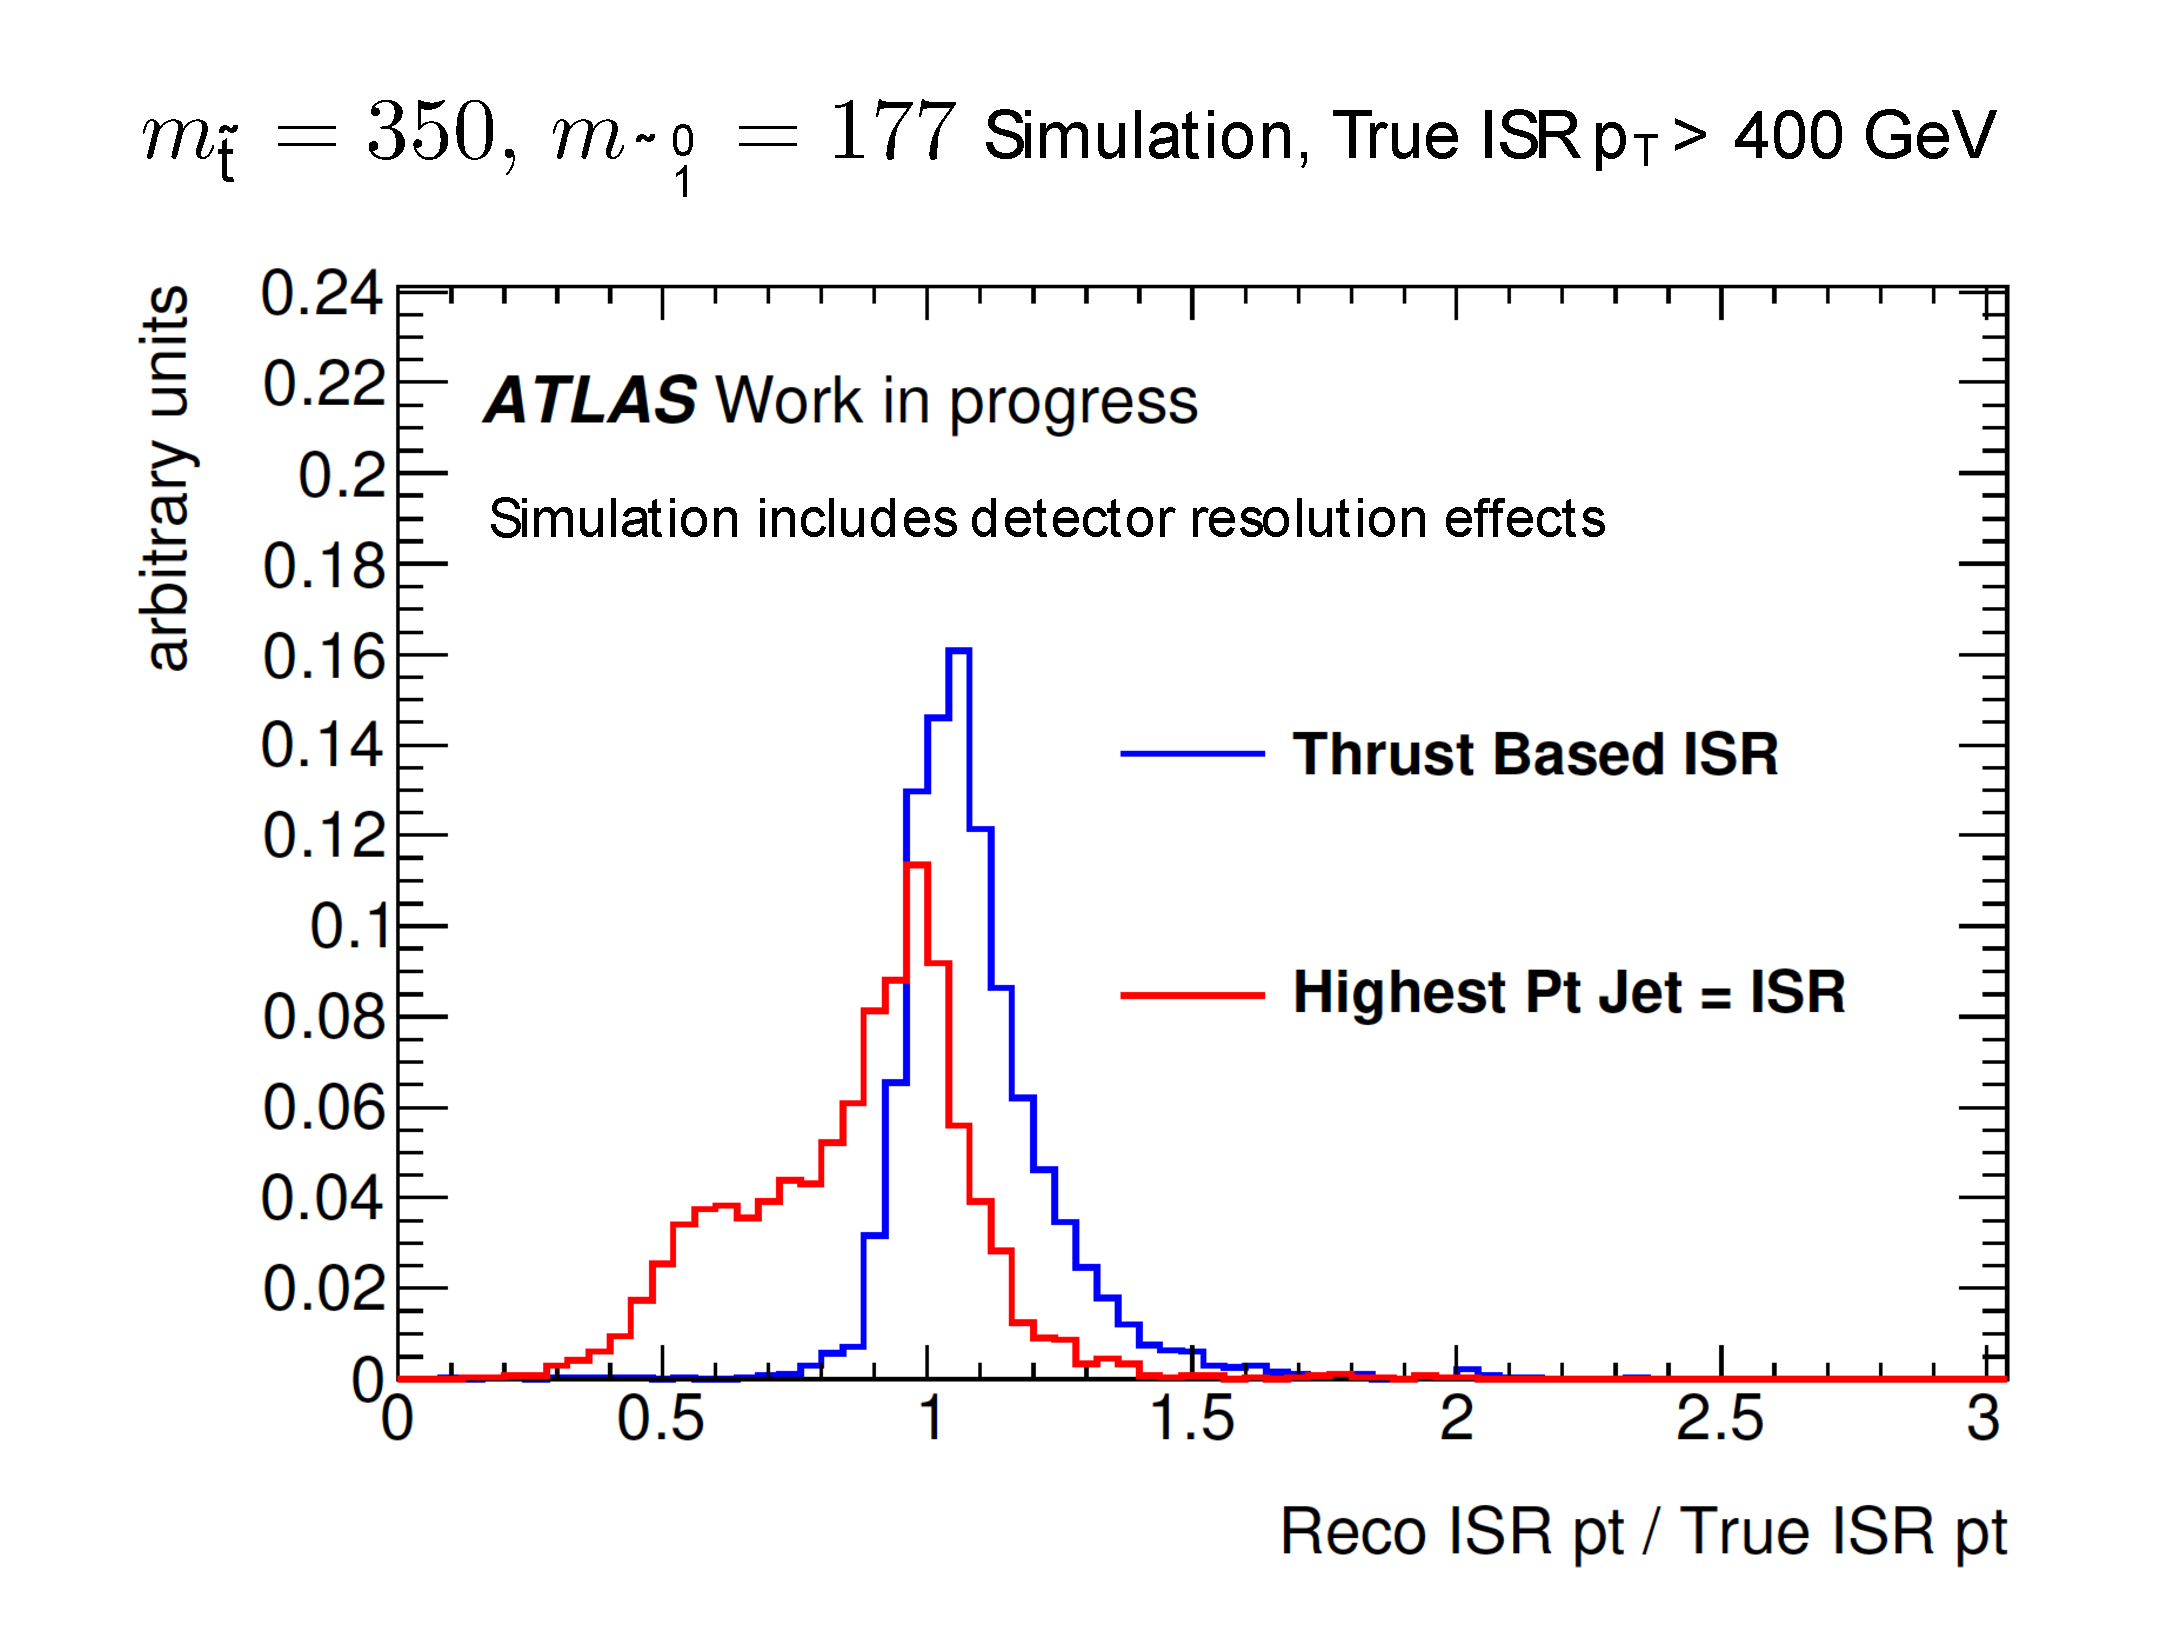
\includegraphics[width=0.75\textwidth]{./figures/strategy/ThrustAlgoEfficiency.eps}
\caption{The distribution of the ratio of reconstructed vs true ISR $\pt$ for the $350$ GeV stop mass and $172$ GeV neutralino mass signal sample.  Only simulations with fully hadronic stop decays and at least $400$ GeV of true ISR $\pt$ are accepted.  The red distribution is formed when the whole ISR system is equated to just the highest $\pt$ jet.  The blue distribution uses the thrust based ISR identification system.  \label{fig:ISRPerformance}}
\end{figure}

\indent A simple and currently popular form of ISR identification is simply the equating the highest $\pt$ jet with the ISR system. The highest $\pt$ jet algorithm is represented by the red distribution in Figure \ref{fig:ISRPerformance}. The single jet algorithm loses $20$-$50$\% of the ISR energy in about $40$\% of events.  This is because the ISR system energy is often split between multiple jets. \\

\indent In comparison, the thrust based ISR identification system is able to capture the whole ISR system consisting of multiple jets.  The fitted gaussian width of the blue peak is $9$\% and this uncertainty includes detector resolution effects.  The gaussian mean is centered about $1.05$.  The reason for this is because a jet originating from a stop will occasionally go in the opposite direction as the $\met$ and be misidentified as an ISR jet.  The $\pt$ of the misidentified sparticle jet tend to be small when compared to the total $\pt$ of the ISR system.  Hence, this misidentification shows up as a $5$\% bias in the reconstructed ISR $\pt$.  Optimization of the ISR identification algorithm shows that this small bias does not impact the sensitivity of the search.  \\

\indent The non-gaussian tail in the blue distribution that extends to a reconstructed over true ISR $\pt$ ratio of $1.5$ is due to energetic ISR jets that go in the same direction as the $\MET$.  In these cases, the ISR jets that are in the same direction as the $\met$ are miss-reconstructed as having originated from a stop.  Only the ISR jets going in an opposite direction to the $\MET$ are reconstructed as ISR jets.  Therefore the reconstructed ISR system fail to partially cancel the $\pt$ of the oppositely facing jets and the reconstructed ISR system has a larger $\pt$ then the true ISR $\pt$.  However, these cases are rare and the non-gaussian tail accounts for less than $15$\% of the events in blue distribution. \\

\section{Kinematic Variables of Initial State Radiation and Sparticle Systems}
\label{Jigsaw:Variables}

\indent Once we separated the event into two hemispheres according the thrust axis as described in section \ref{Jigsaw:ISR} we can construct a number of kinematic variables that captures different features of the two hemispheres.  These variables are listed below. \\

\begin{description}
\item [\boldmath \NbV:] number of b-tagged jets associated with the sparticle hemisphere.
\item [\boldmath \NjV:] number of jets associated with the sparticle hemisphere.
\item [\boldmath \pTSBZero:] $\pt$ of the leading b-tagged jet in the sparticle hemisphere.
\item [\boldmath \pTjV:] $\pt$ of the fourth highest $\pt$ jet in the sparticle hemisphere.
\item [\boldmath \MS:] transverse mass of the whole sparticle system and $\met$.
\item [\boldmath \PTISR:] $\pt$ of the ISR system.
\item [\boldmath \dphiISRI:] angular separation in $\phi$ of the ISR and the $\met$ (evaluated in the transverse CM frame).
\item [\boldmath \RISR:] ratio between $\met$ and $\PTISR$ (evaluated in transverse CM frame).
\end{description}

\indent $\NjV$ and $\NbV$ quantify the jet multiplicity in the sparticle system.  $\pTSBZero$, $\pTjV$, $\MS$ and $\PTISR$ quantify the amount of energy in the sparticle and ISR hemispheres.  Finally, $\dphiISRI$ and $\RISR$ describe the correlation between the ISR system and the $\MET$ in direction and magnitude.  All of these variables will be used to separate signal from background in the signal region described in detail in chapter \ref{chap:SignalRegion}. \\

